\documentclass[letterpaper]{l3doc}

\hypersetup{urlcolor = teal, filecolor = violet}
\usepackage[mono = false]{libertine}
\usepackage{pdfpages,hologo,framed}
\hologoFontSetup{general = \sffamily}
\FrameSep = 0pt
\usepackage[fontset = none]{ctex}
\setCJKmainfont[BoldFont = *-Medium]{LXGW WenKai}
\setCJKsansfont[BoldFont = *-Medium]{LXGW WenKai}
\setCJKmonofont[BoldFont = *-Medium]{LXGW WenKai Mono}
\usepackage[os = mac]{menukeys}
\AddToHook{env/function/before}{\vspace{-.3\baselineskip}}
\AddToHook{env/syntax/after}{\vspace{-.2\baselineskip}}

\title
{
  \bfseries\cls{litetable} 文檔類:多彩嘅課程表
  \footnote{\url{https://github.com/xiamyphys/litetable}}
}
\author
{
  夏明宇 \texttt{<\href{mailto:xiamyphys@gmail.com}{xiamyphys@gmail.com}>}
  \thanks{\href{https://github.com/ljguo1020}{郭李軍}開發咗讀取 \meta{left} -> \meta{right} 型資料結構糢塊同低版本 \hologo{TeX} Live 相容糢塊.}
}
\date{Version 3.1D, \today}

\begin{document}

\maketitle

\section{介紹}

\cls{litetable} 文檔類提供咗個多彩嘅課程表設計,基於 \cls{article} 文檔類,由 \pkg{expl3} 和 \pkg{tikz} 構建. 相容發行版 \hologo{TeX} Live 2019 同更高版本,喺 \hologo{pdfLaTeX} 同 \hologo{XeLaTeX} 編譯器下均可正常運行. 本文檔系 \cls{litetable} 文檔類嘅用户手冊放,手冊放同時有 \href{./litetable-en.pdf}{英文} 同 \href{./litetable-cn.pdf}{官話} 版本\footnote{\href{https://qm.qq.com/q/RyssAhG4qy}{QQ Group: 760570712}}.

\section{載入 \cls{litetable} 並建置課程表框架}

同載入其他文檔類一樣,只令寫下

\begin{framed}
  \begin{verbatim}
    \documentclass {litetable}
  \end{verbatim}
\end{framed}

如需輸入中文,可自行載入 \pkg{ctex} 宏包並設置字型.

\begin{function}{\timelist,\weeklist}
  \begin{syntax}
    \cs{timelist} \oarg{rows} \marg{list}            \cs{timelist} \marg{list} \oarg{rows}
    \cs{weeklist} \oarg{default weeks} \marg{list}   \cs{weeklist} \marg{list} \oarg{default weeks}
  \end{syntax}

  命令 \cs{timelist} 嘅可選參數可強制設定課程表嘅行數,命令 \cs{weeklist} 嘅可選參數可設定預設嘅星期數目並會喺每個課程盒子嘅右下角顯示. 兩個命令嘅強制參數均接受數組,可分別就系課程表嘅左側添加時間表、喺課程表嘅頂部添加對應寬度比例嘅工作日. 輸入數組嘅用例見Appendix \ref{mwe}.
  
  若命令 \cs{timelist} 中時間數組數字大於可選參數接受值,就多餘嘅時間數組將畀忽略,並返回一個警告. 如果只系課程表左側添加一部序號,令強制參數為空即可.
\end{function}

\begin{function}{\more}
  \begin{syntax}
    \cs{more} \marg{comment}
  \end{syntax}

  此命令可喺頁面嘅嘅右下角添加備注.
\end{function}

\begin{function}{\maketable}
  \begin{syntax}
    \cs{maketable} \oarg{keyvals} \marg{title} \oarg{keyvals}
  \end{syntax}

  此命令可建置一個空白嘅課程表框架,使喺命令 \cs{timelist},\cs{weeklist} 同 \cs{more} 後,並喺帶有 \cmd{[remember picture, overaly]} 選項嘅 \env{tikz} 環境中執行. 可選引數接受鍵 \keys{\cmdmac~color} \keys{\cmdmac~sem},可分別就喺設置課程表框架嘅背景色同喺頁面嘅嘅右度角添加學期,鍵 \keys{\cmdmac~color} 嘅默認值為 \cmd{gray}. 強制參數可設定標題.
\end{function}

\section{添加課程盒子}

\begin{function}{\course}
  \begin{syntax}
    \cs{course} \oarg{keyvals} \marg{start number} \oarg{keyvals} \marg{end number} \oarg{keyvals}
  \end{syntax}

  \cs{course} 命令可喺當前工作日添加課程盒子,要喺命令 \cs{maketable} 後,並喺帶有 \cmd{remember picture,overaly} 選項嘅 \env{tikzpicture} 環境中執行.
  
  此命令嘅可選參數接受下列鍵:\keys{\cmdmac~color} \keys{\cmdmac~subject} \keys{\cmdmac~location} \keys{\cmdmac~teacher} \keys{\cmdmac~weeks}. 鍵 \keys{\cmdmac~color} 默認值為 \cmd{teal},鍵 \keys{\cmdmac~weeks} 默認值由命令 \cs{weeklist} 嘅可選參數決定. 第一個同第二個強制參數勒分別為課程嘅開始同結束序號. 命令嘅用例見Appendix \ref{mwe}.

  \begin{itemize}
    \item 若課程盒子高度得一格,即$\marg{start number} = \marg{end number}$,就鍵 \keys{\cmdmac~location} 同 \keys{\cmdmac~teacher} 嘅值將輸出喺同一行並以逗號 (,) 隔,鍵 \keys{\cmdmac~weeks} 嘅值將會隱藏.
    \item 若鍵 \keys{\cmdmac~location} 同 \keys{\cmdmac~teacher} 均未賦值,就鍵 \keys{\cmdmac~subject} 嘅值將輸出喺課程盒子中心.
    \item 超出課程表工作日範圍嘅課程盒子將唔會顯示,只會返回一條警告.
  \end{itemize}
\end{function}

\begin{function}{\newday}
  \begin{syntax}
    \cs{newday} \oarg{integral value}
  \end{syntax}

  此命令有一個可選參數,可令其後面添加嘅課程盒子後移 \meta{intergal value} 個工作日. 可選參數嘅默認值為\cmd{1},即後移\cmd{1}個工作日.
\end{function}

\clearpage
\appendix

\section{最小工作範例}\label{mwe}

此MWE建置嘅課程表有13行但系得前12行标注时间,課程表顶部共有五个工作日,工作日之间嘅宽度比例为$4:5:4:6:5$,键 \keys{\cmdmac~weeks} 嘅默认值畀赋为 \cmd{Weeks 1 - 16}. 添加咗註解同兩個課程盒子.

\begin{framed}
  \begin{verbatim}
    \documentclass{litetable}

    \begin{document}

    \timelist [ 13 ]
      {
        08:05 -> 08:50, 08:55 -> 09:40, 10:00 -> 10:45, 10:50 -> 11:35,
        11:40 -> 12:25, 13:30 -> 14:15, 14:20 -> 15:05, 15:15 -> 16:00,
        16:05 -> 16:50, 18:30 -> 19:15, 19:20 -> 20:05, 20:10 -> 20:55
      }
    \weeklist [ Weeks 1 - 16 ]
      {
        Mon -> 4, Tue -> 5, Wed -> 4, Thu -> 6, Fri -> 5
      }
    \more { Author: Mingyu Xia \& Lijun Guo }

    \begin{tikzpicture} [ remember picture, overlay ]
      \maketable
      \course [ subject = Keep on {\TeX}ing ] {10} {11}
      \newday
      \course [ color = DarkSlateGray, subject = litetable,
                location = Hong Kong, teacher = M.Y. Xia
              ] {8} {8}
    \end{tikzpicture}

    \end{document}
  \end{verbatim}
\end{framed}

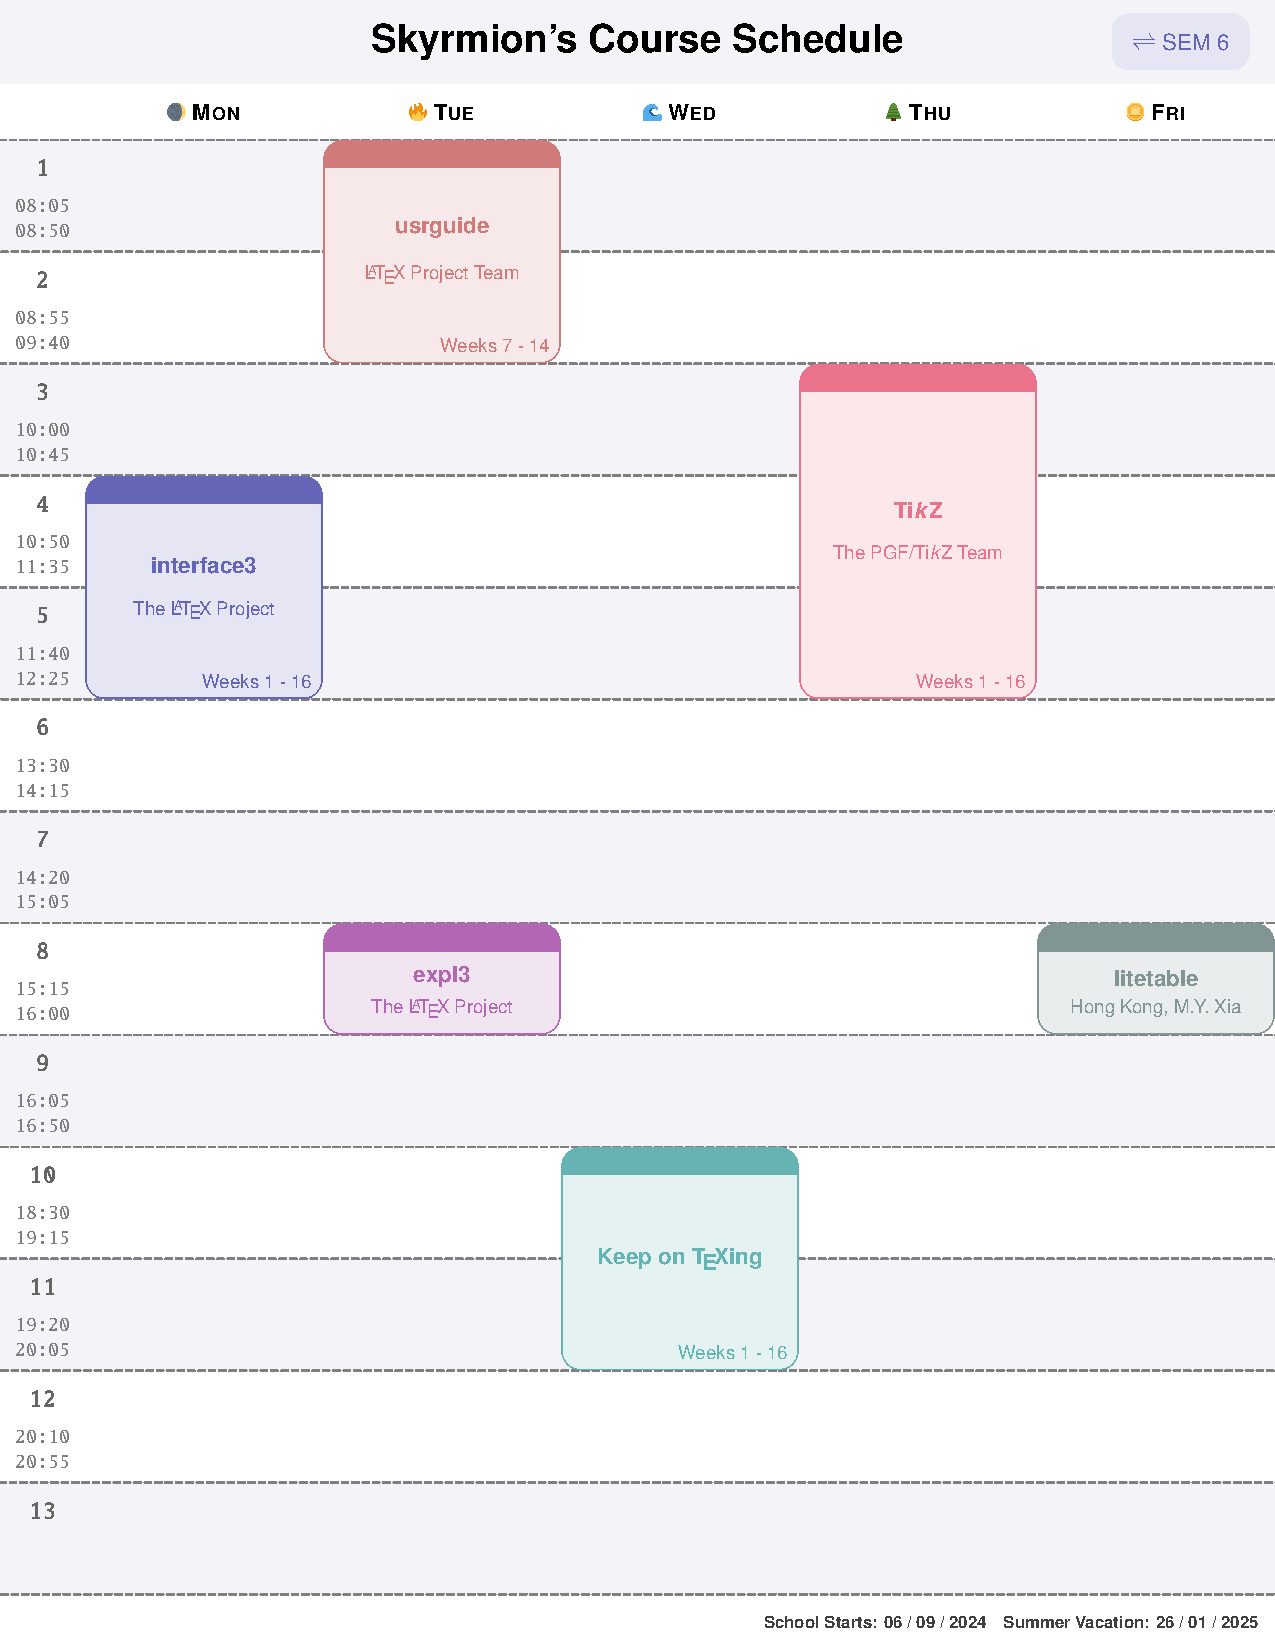
\includepdf[pages = 1]{litetable-demo.pdf}

\end{document}

% End of file litetable-hk.tex
